\documentclass{article} % For LaTeX2e
\usepackage{nips_adapted}
\usepackage{hyperref}
\usepackage{url}
\usepackage{amsmath}
\usepackage{graphicx}
\usepackage{amssymb}
\usepackage{hyperref}
\usepackage{subfig}
\hypersetup{
    colorlinks=true,
    linkcolor=blue,
    filecolor=magenta,      
    urlcolor=blue,
}

\usepackage{listings}
\usepackage{color}

\lstset{frame=tb,
	language=Java,
	aboveskip=3mm,
	belowskip=3mm,
	showstringspaces=false,
	columns=flexible,
	basicstyle={\small\ttfamily},
	numbers=none,
	breaklines=true,
	breakatwhitespace=true,
	tabsize=3
}

\definecolor{applegreen}{rgb}{0.55, 0.71, 0.0}
\definecolor{azure(colorwheel)}{rgb}{0.0, 0.5, 1.0}
\definecolor{awesome}{rgb}{1.0, 0.13, 0.32}
\definecolor{ao(english)}{rgb}{0.0, 0.5, 0.0}
\definecolor{darkmidnightblue}{rgb}{0.0, 0.2, 0.4}

\title{CS 639A Progress Report 2}

\author{
Sumit Lahiri \\
19111274 \\
\And
Group No\\
1\\
\And
Amit Kumar Sharma \\
20111012\\
}

% The \author macro works with any number of authors. There are two commands
% used to separate the names and addresses of multiple authors: \And and \AND.
%
% Using \And between authors leaves it to \LaTeX{} to determine where to break
% the lines. Using \AND forces a linebreak at that point. So, if \LaTeX{}
% puts 3 of 4 authors names on the first line, and the last on the second
% line, try using \AND instead of \And before the third author name.

\newcommand{\fix}{\marginpar{FIX}}
\newcommand{\new}{\marginpar{NEW}}
\usepackage{xcolor}

\nipsfinalcopy


\begin{document}

\maketitle

\section*{Reinforcement Learning Stage Report : Pre-RL \& RL Stage}
After completing the \textbf{stage 1} work, we moved to the \textbf{stage 2} work. Our first task to start modifying and preparing the various programs and \textbf{scripts}, \textbf{manifests} \& \textbf{libraries} needed for both the \textbf{\href{https://github.com/ashish-gehani/OCCAM}{OCCAM}} tool and \textbf{\href{https://github.com/aspire-project/chisel}{Chisel}} tool. These tools already had picked up some benchmark runs, so our first trial was to prepare according to the following benchamarks for the tools, namely \textbf{\href{https://github.com/lahiri-phdworks/chisel-bench}{Chisel Tool benchmarks}} , \textbf{\href{https://github.com/lahiri-phdworks/OCCAM-Benchmarks}{OCCAM Tool benchmarks}} \& \textbf{\href{https://github.com/ashish-gehani/OCCAM-Benchmarks}{Trimmer Tool benchmarks}}.  

These benchmarks needed modification interms of running it against updated \textbf{\href{https://github.com/SRI-CSL/gllvm}{gllvm}}, \textbf{\href{https://github.com/SRI-CSL/whole-program-llvm}{wllvm}} \& \textbf{\href{https://github.com/lahiri-phdworks/llvm-project/tree/release/10.x}{llvm-10}}. There were a few other tools and frameworks that we had to install and test inorder to run the debloating tools on the current benchamarks as described. 

We devised that we can split the runs and the debloating process for comparision on three seperate pipelines namely, \textbf{chisel-tool}, \textbf{occam-tool}
\& \textbf{deepoccam-tool} pipeline. Our intension is to run each tool seperately on a single example and then compare them against the \textbf{\href{https://github.com/michaelbrownuc/GadgetSetAnalyzer}{GadgetSetAnalyser}}. We list below the work we did on each pipeline for \textbf{Week-2} \& \textbf{Week-3} of our development. We lag behind in the \textbf{Week-4} activity, which we intend to migate in the last week hopefully. 

\section*{\color{darkmidnightblue} Pipeline : Chisel Tool} 
We share a brief information about the tool. \textbf{Chisel} tool works by learning a \textbf{policy} for \textbf{delta debugging} by \textbf{reinforcement learning} which guarantees \textbf{1-minimal P*} \& $\textbf{$O(|P|^2)$}$ runtime. The abstraction is that a \textbf{markov decision process} is being used to model the \textbf{reinforcement learning} problem for meaningful \textbf{guidance} to learn the \textbf{policy} in a better way. All global declarations, variables, functions etc. are first reduced by the delta-debugging principle as state above and thereafter local variables, loop declarations and arguments to functions are optimized. After both the local and global level reductions are done, \textbf{Chisel} invokes a run of the \textbf{global level reduction} again and repeats the process continually until the \textbf{1-minimal P*} version of the program is found. 
\begin{itemize}
	\item Install and preparation work for \textbf{\href{https://github.com/lahiri-phdworks/chisel-bench}{Chisel Tool benchmarks}} and \textbf{wllvm}. The code was dated so we made the modifications to run and process it further. 
	\item We wrote specification for the script used by \textbf{\href{https://github.com/aspire-project/chisel}{Chisel}} tool as in \href{https://dl.acm.org/doi/10.1145/3243734.3243838}{Paper 1} in terms of the three parts of the scripts namely \textbf{\texttt{compile()}}, \textbf{\texttt{desired()}} \& \texttt{\textbf{undesired()}} for some of the benchmark runs.
	\item Generating a proper binary after reduction was difficult given we had some missing \textbf{linked shared objects} \& \textbf{undefined symbols} issue. We resorted to building and modifiying \textbf{Chisel} tool and the benchmark examples in \textbf{docker} \textbf{\href{https://hub.docker.com/r/prodrelworks/chisel-tool}{containers}} against the correct tools and setup for \textbf{\href{https://github.com/michaelbrownuc/GadgetSetAnalyzer}{GadgetSetAnalyser}}
	\item Prepare \textbf{\href{https://github.com/michaelbrownuc/GadgetSetAnalyzer}{GadgetSetAnalyser}} to \textbf{ROP Gadgets} only. We plotting the results properly and extend it to show the total number of unqiue gadgets. 
	\item \textbf{\color{ao(english)} We have completed a basic run of our pipeline on Chisel Tool}
\end{itemize}

\begin{lstlisting}
	Running delta debugging - Size: 0
	Start local reduction
	Reduce main at ./test/function1/function1.c
	Reduce File: ./test/function1/function1.c
	Iteration 1 (Word: 4)
	Start global reduction
	Running delta debugging - Size: 0
	Start local reduction
	Reduce main at ./test/function1/function1.c
	...
\end{lstlisting}

Final Results from the tool. We show a partial dump here. 

\begin{lstlisting}
	====================================================
							Report                       
	====================================================
		Total Time :                                1.1s
		Oracle Time :                               0.5s
		Learning Time :                             0.1s
		Global Success Ratio :               0% ( 0 / 0)
		Local Success Ratio :              100% ( 3 / 3)
		Functions (Original) :                         1
		Statements (Original) :                        4
		Functions (Reduced) :                          1
		Statements (Reduced) :                         2
\end{lstlisting}

\begin{figure}%
	\centering
	\subfloat[\centering Chisel Tool Run : Function 1 Example]{{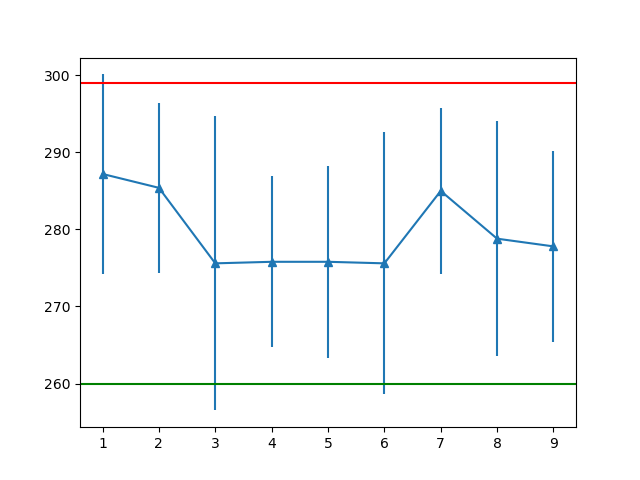
\includegraphics[width=6cm]{chisel_graph_5_10.png} }}%
	\qquad
	\subfloat[\centering Chisel Tool Run : Function 1 Example]{{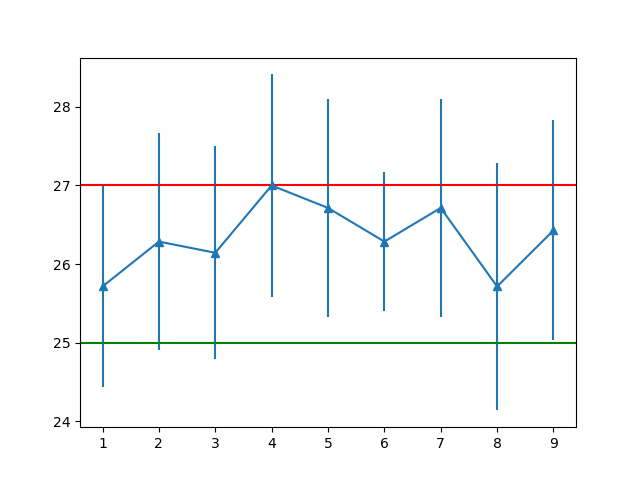
\includegraphics[width=6cm]{chisel_graph_7_10.png} }}%
	\caption{Chisel Tool runs on \textbf{\texttt{two examples}}. \textbf{\color{red} Before} and \textbf{\color{ao(english)} After} debloating.}%
	\label{fig:example1}%
\end{figure}

\section*{\color{darkmidnightblue} Pipeline : OCCAM Tool} 
\textbf{OCCAM} is a whole-program partial evaluator for LLVM bitcode that aims at debloating programs and shared/static libraries running in a specific deployment context.
\begin{itemize}
	\item Prepared the examples and the benchmark codes for \textbf{OCCAM} runs. 
	\item We had to refactor the code and modify it for \textbf{docker} \textbf{\href{https://hub.docker.com/r/prodrelworks/occam10}{containers}} run. Most of the work was to link it properly with it's dependencies and build it for the base level run. 
	\item Running the tool against some examples in the \textbf{OCCAM} repository. We ran our modified tool in this case.
	\item Running the tool in following \textbf{\texttt{none}}, \textbf{\texttt{aggressive}}, \textbf{\texttt{bounded}} \& \textbf{\texttt{onlyonce}} modes. 
	We shall detail out the runs and the options in \textbf{report} we submit.  
	\item We ran the \textbf{OCCAM} tool for run on \textbf{bzip2}, \textbf{httpd}, \textbf{tree} and many other programs as listed in the benchmarks.
	\item Compared to \textbf{Chisel} as we ran \textbf{OCCAM} on some sample \textbf{\texttt{C}} \& \textbf{\texttt{C++}} code.
	\item Refactored the code to support the new version for \textbf{\href{https://github.com/seahorn/sea-dsa}{sea-dsa}} for the \textbf{\texttt{--use-pointer-analysis}} option needed to do futher \textbf{\texttt{dce}} on the code and also to support \textbf{\texttt{--ai-dce}}
\end{itemize}

A sample run of the tool where we show that \textbf{OCCAM} tool has specialized some of the \textbf{\color{ao(english)} call-sites} 
\begin{lstlisting}
[23/11/2020 19:18:51] STARTED runbench
[23/11/2020 19:18:51] RUN make on tree
Running slash with options ['./build.sh', '--disable-inlining', '--enable-config-prime']
[23/11/2020 19:18:53] RUN ./build.sh --disable-inlining --enable-config-prime on tree
[23/11/2020 19:18:55] FINISHED runbench

Program Reduction: (B:before and A:after OCCAM with --disable-inlining --enable-config-prime)

Program B Fun  A Fun  %Fun Red  B Ins  A Ins  %Ins Red  B Mem Ins  A Mem Ins %Mem Ins Red
tree       52     32        38  7442   4110         44       1658        810           51
\end{lstlisting}

Results for \textbf{\texttt{GNU Tree}} program on \textbf{OCCAM} tool on \textbf{llvm-10} after required modifications \& \textbf{\color{ao(english)} successful} build.  We show a partial dump here. 

\begin{lstlisting}
Statistics for tree before specialization
[CFG analysis]
52 Number of functions
0 Number of specialized functions
0 Number of bounced functions added by devirt
1458 Number of basic blocks
7442 Number of instructions
1051 Number of direct calls
845 Number of external calls
15 Number of indirect calls
0 Number of unknown calls
43 Number of loops   
0 Number of bounded loops
[Memory analysis]
1944 Number of memory instructions
286 Statically safe memory accesses
1658 Statically unknown memory accesses

Statistics for tree after specialization
[CFG analysis]
40 Number of functions
0 Number of specialized functions
0 Number of bounced functions added by devirt
1845 Number of basic blocks
8957 Number of instructions
1257 Number of direct calls
1167 Number of external calls
15 Number of indirect calls
0 Number of unknown calls
66 Number of loops   
0 Number of bounded loops
[Memory analysis]
2222 Number of memory instructions
348 Statically safe memory accesses
1874 Statically unknown memory accesses
\end{lstlisting}

Results for \textbf{\texttt{GNU bzip2}} program on \textbf{OCCAM} tool on \textbf{llvm-10} after required modifications \& \textbf{\color{ao(english)} successful} build.  

\begin{lstlisting}
Statistics for bzip2 before specialization
[CFG analysis]
108 Number of functions
0 Number of specialized functions
0 Number of bounced functions added by devirt
3223 Number of basic blocks
26718 Number of instructions
678 Number of direct calls
304 Number of external calls
0 Number of assembly calls
20 Number of indirect calls
0 Number of unknown calls
161 Number of loops   
0 Number of bounded loops
[Memory analysis]
12589 Number of memory instructions
8304 Statically safe memory accesses
4285 Statically unknown memory accesses

Statistics for bzip2 after specialization
[CFG analysis]
94 Number of functions
0 Number of specialized functions
0 Number of bounced functions added by devirt
2334 Number of basic blocks
19877 Number of instructions
672 Number of direct calls
293 Number of external calls
0 Number of assembly calls
20 Number of indirect calls
0 Number of unknown calls
180 Number of loops   
18 Number of bounded loops
[Memory analysis]
5187 Number of memory instructions
486 Statically safe memory accesses
4701 Statically unknown memory accesses
\end{lstlisting}

\section*{\color{darkmidnightblue} Pipeline : DeepOCCAM Tool} \textbf{DeepOCCAM} does specialization and optimizations with the help of \textbf{OCCAM} tool. The \textbf{DeepOCCAM} tool is different from \textbf{OCCAM} in the sense that \textbf{DeepOCCAM} does deep learning implemented in \textbf{PYTORCH} to learn a policy. The model also keeps information of the decisions made on each iteration to update the policy via \textbf{\texttt{def push\_to\_memory(self, memory)}}. We found a \textbf{\href{https://github.com/nhamlv-55/OCCAM/tree/mlpolicy}{half-implemented code}} repository which belongs to one of the authors for \textbf{DeepOCCAM} paper. The tool doesn't link, build or run on the current platform that we are using. It gave us insights on implementing some of the parts in the code that we are developing as an extension on \textbf{OCCAM} to develop \textbf{DeepOCCAM}.
\begin{itemize}
	\item Modified code in base \textbf{OCCAM} tool to collect \textbf{RL} related features and added support for \textbf{gRPC} server which can run and communicate with the \textbf{PyTorch} RL Model running as client. \textbf{\color{red} (We are facing linking issues here.)}
	\item Implemented a \textbf{deep reinforcement learning model} from the insights we got from the \textbf{\href{https://github.com/nhamlv-55/OCCAM/tree/mlpolicy}{half-implemented code}}. 
	\item We setup a \textbf{docker} based \textbf{\href{https://hub.docker.com/r/prodrelworks/deepoccam8}{deepoccam combined-tools}} container pipeline to build, run and debloat an example \textbf{\color{blue} code repository}. The \textbf{training} part happened outside the docker, we just saved and extracted the model for later use in \textbf{\href{https://hub.docker.com/r/prodrelworks/deepoccam8}{deepoccam-combined-tools}} container. 
	\item We had to modify the way the tool was plotting and processing some the feature vectors. We used \textbf{\texttt{Adam Optimization}}, \textbf{\texttt{ReLU}} functions, \textbf{\texttt{Softmax}}, \textbf{\texttt{torch.nn GRU}} neural net for \textbf{\texttt{inst2vec}} \& \textbf{\texttt{Linear fully-connected}} layers etc. for implementing the \textbf{\texttt{ML}} part of \textbf{DeepOCCAM} tool.
	\item We are yet to complete the training phase over \textbf{gRPC} connection where the \textbf{OCCAM} tool runs and gives the data for the \textbf{\texttt{RL Features}}. We are currently running \textbf{OCCAM} tool in \textbf{non-gRPC} mode and training the tool based on some 
	\textbf{\texttt{metadata.json}} files we got in the \textbf{\href{https://github.com/nhamlv-55/OCCAM/tree/mlpolicy}{half-implemented code}} repository. 
	\item The \textbf{\href{https://github.com/nhamlv-55/OCCAM/tree/mlpolicy}{half-implemented code}} repository really helped us in correcting and implementing some of the design decisions we made in the early implementation of the \textbf{DeepOCCAM} tool from \textbf{OCCAM}.
	\item As before, we are developing from \textbf{OCCAM} tool repository to build \textbf{DeepOCCAM} after gaining some insights and \textbf{metadata} files from \textbf{\href{https://github.com/nhamlv-55/OCCAM/tree/mlpolicy}{half-implemented code}} we got. 
\end{itemize}

\section*{\color{darkmidnightblue} Metrics Testing : COP, ROP \& JOP Gadgets} 
\textbf{Call Oriented programming (COP)},\textbf{Jump Oriented programming (JOP)} and \textbf{Return Oriented Programming (ROP)} are \textbf{computer security exploitation} techniques. The hacker uses the binary instructions to combine some sort of short sequences of instructions which are commonly called \textbf{gadgets} using return section code in the stack and make \textbf{unwanted} stack sections directly \textbf{executable}. The gadgets like COP, ROP \& JOP \textbf{hijack} the actual control flow of the program and once the control is disturbed, hacker can make use of this \textbf{opportunity} to attack the system. Therefore, it is necessary to keep these gadgets as minimum as possible. While \textbf{debloating} the program \textbf{reduces} the number of gadgets, it is still not guaranteed that the attack is prevented but it \textbf{minimizes} the attack surface to a certain extent.

It is extremely important to keep track of the metrics of \textbf{gadgets} as these metrics when used to learn a RL policy will help in maximizing the rewards which in turn reduces the \textbf{code attack} surface. So while testing \textbf{DeepOCCAM}, these gadgets counts need to be tracked. We use the \textbf{number} of \textbf{gadgets} we get by running each tool namely \textbf{Chisel}, \textbf{trimmer}, \textbf{OCCAM} or our implementation of \textbf{DeepOCCAM} as a \textbf{\color{ao(english)} reasonably important} metric of comparision. 

\begin{figure}%
	\centering
	\subfloat[\centering DeepOOCAM Run 20 : \textbf{\texttt{bzip2}} training]{{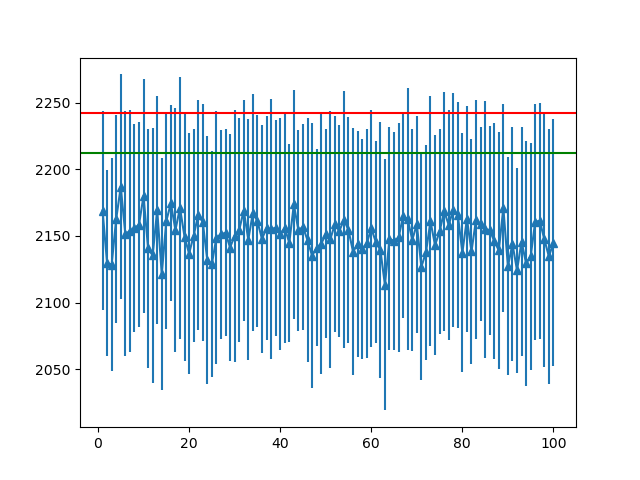
\includegraphics[width=6cm]{deepoccam_run1_example.png} }}%
	\qquad
	\subfloat[\centering DeepOOCAM Run 50 : \textbf{\texttt{bzip2}} training]{{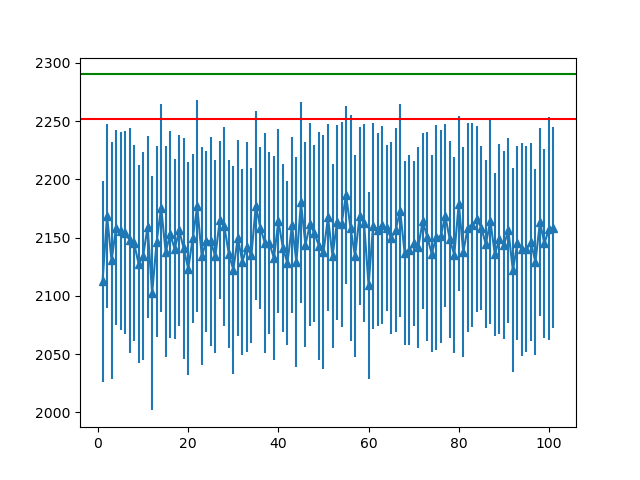
\includegraphics[width=6cm]{deepoccam_run2_example.png} }}%
	\caption{DeepOCCAM Tool runs on \textbf{\texttt{bzip2}}. \textbf{\color{red} Before} and \textbf{\color{ao(english)} After} debloating}%
	\label{fig:example}%
\end{figure}

\section*{\color{darkmidnightblue} Pending Works} 
A word on \textbf{Trimmer}, \textbf{OCCAM} also uses partial evaluation concept like \textbf{Trimmer} for specializing applications but it is less aggressive compared to the  \textbf{Trimmer} because it does not include \textbf{\texttt{loop unrolling}} and \textbf{\texttt{constant propagation}} for optimizations. 

We have to complete some parts of the \textbf{DeepOCCAM} tool in the \textbf{RL Model} part. \textbf{We are yet to run the three tools on common examples to get enough data for a good comparision report and smooth running implementation}. We may have to skip the \textbf{gRPC} based implementation upon a \textbf{time crunch}. Building, fixing, refactoring and developing the tools for a smooth run took \textbf{\color{red} more time than we actually expected}. 

\section*{Code \& Docker Links for Tools}
\begin{itemize}
	\item OCCAM Tool : \textbf{\href{https://github.com/lahiri-phdworks/OCCAM} {https://github.com/lahiri-phdworks/OCCAM}}
	\item OCCAM Test \& Benchmarks : \textbf{\href{https://github.com/lahiri-phdworks/OCCAM-Benchmarks} {https://github.com/SRI-CSL/OCCAM-Benchmarks}}
	\item Chisel-Bench : \textbf{\href{https://github.com/lahiri-phdworks/chisel-bench} {https://github.com/lahiri-phdworks/chisel-bench}}
	\item Chisel Tool : \textbf{\href{https://github.com/lahiri-phdworks/chisel} {https://github.com/lahiri-phdworks/chisel}}
	\item Inst2Vec : \textbf{\href{https://github.com/lahiri-phdworks/ncc} {https://github.com/lahiri-phdworks/ncc}}
	\item Binary GSA Testing Tool : \textbf{\href{https://github.com/michaelbrownuc/GadgetSetAnalyzer} {https://github.com/michaelbrownuc/GadgetSetAnalyzer}}
	\item Docker Images (recent ones) : \textbf{\href{https://hub.docker.com/u/prodrelworks} {https://hub.docker.com/u/prodrelworks}}
\end{itemize}

\end{document}


